% ENCORE — IEEE Transactions on Smart Grid submission
% Budget: 10–10.5 pages total, <=30 references (owner constraint, 2026-06-11).
% Section allocation (target): I 1.2 | II 0.8 | III 0.8 | IV 1.2 | V 1.7 | VI 1.8
%                              | VII 2.2 | VIII 0.4 | refs 0.7  ~= 10.3 pp
\documentclass[journal]{IEEEtran}

\usepackage{amsmath,amssymb,amsthm}
\usepackage{graphicx}
\usepackage{booktabs}
\usepackage{multirow}
\usepackage[caption=false]{subfig}
\usepackage{xcolor}

\graphicspath{{../results/phase6/}{../results/phase1/}{../results/phase2/}}

\newtheorem{theorem}{Theorem}
\newtheorem{lemma}{Lemma}
\newtheorem{remark}{Remark}
\newtheorem{assumption}{Assumption}

\newcommand{\Ft}{\widetilde{F}}
\newcommand{\Wsafe}{\mathcal{W}^{\mathrm{s}}}
\newcommand{\Wdel}{\mathcal{W}^{\mathrm{d}}}
\newcommand{\epss}{\varepsilon_{\mathrm{s}}}
\newcommand{\epsd}{\varepsilon_{\mathrm{d}}}
\newcommand{\todo}[1]{\textcolor{red}{[TODO: #1]}}

\begin{document}

\title{Certified Cooling-Side Flexibility for Liquid-Cooled AI Data Centers:
Context-Dependent Envelopes with End-to-End Delivery Guarantees}

\author{Jiachen~Shen% <-- author block to be completed by owner
\thanks{Manuscript received \todo{date}. The author is with \todo{affiliation}.}}

\maketitle

\begin{abstract}
\todo{Abstract drafted last (Sec.~order: VII $\to$ V--VI $\to$ IV,III $\to$ II,I).}
\end{abstract}

\begin{IEEEkeywords}
Data centers, demand response, flexibility envelope, liquid cooling, day-ahead
markets, conformal prediction, robust control.
\end{IEEEkeywords}

% =====================================================================
\section{Introduction}\label{sec:intro}
\todo{Sec.~I drafted fourth.}

% =====================================================================
\section{Related Work}\label{sec:related}
\todo{Sec.~II drafted fourth.}

% =====================================================================
\section{Problem Setting}\label{sec:setting}
\todo{Sec.~III drafted third.}

% =====================================================================
\section{Plant Model}\label{sec:plant}
\todo{Sec.~IV drafted third.}

% =====================================================================
\section{The Certified Flexibility Envelope}\label{sec:envelope}
\todo{Sec.~V drafted second (Thm.~1, virtual battery, whole-hour product semantics).}

% =====================================================================
\section{Two-Stage Offering with Delivery Guarantees}\label{sec:offering}
\todo{Sec.~VI drafted second (nested sets, Thm.~2--3, $e_0$ lemma, offering).}

% =====================================================================
\section{Case Study}\label{sec:casestudy}

\subsection{Data, Calibration, and Protocol}\label{sec:cs-setup}
All experimental inputs are measured data; no synthetic disturbance process
appears anywhere in this section. The thermal plant is calibrated to the
liquid-cooled hall of~\cite{gheni26} (Sec.~\ref{sec:plant}); its parameters are
frozen before any market experiment. Heat-load uncertainty comes from the
Alibaba PAI GPU-cluster trace~\cite{weng22} (2.0\,M workers over 46 usable
days), mapped to a 1\,MW$_{\mathrm{IT}}$ hall profile at 5-min resolution.
Day-ahead heat forecasts use only information available at the 12:00 issue
time: the survival-weighted load of jobs already running plus an
hour-of-day/level regression for short-job churn, both fit causally
(Sec.~\ref{sec:offering}). Weather is the KIAH (Houston Intercontinental) ASOS
record, paired with \emph{archived} day-ahead numerical-weather-prediction
dew-point forecasts,\footnote{Open-Meteo previous-runs archive,
\texttt{dew\_point\_2m\_previous\_day1}; measured day-ahead residual standard
deviation 2.0\,K at this site. Price and weather data accessed via
\texttt{gridstatus} and the Iowa Environmental Mesonet.} so both the
disturbance-set calibration and every simulated day use real forecast errors.
Prices are ERCOT day-ahead SPPs, 15-min real-time SPPs, and ECRS clearing
prices for the Houston hub.

The evaluation protocol separates design from validation. The trace is split
into day blocks: the first two thirds (\emph{fit block}) calibrate forecasts,
conformal disturbance sets, and every design constant (feedback gain, face
allocation, $\epsd$); the final third (\emph{evaluation block}) is replayed
exactly once, in closed loop, over ten 2024 ERCOT weeks spanning all seasons
(including Winter Storm Heather) $\times$ 20 random seeds. All controllers in a
given seed face identical realized disturbances and activation calls.
Every figure and table regenerates from committed configurations and seeds via
a single \texttt{make figures} invocation.

We compare six participants: \textbf{B1} non-participating plant; \textbf{B2}
offers from the \emph{deterministic} envelope $F$ (no uncertainty);
\textbf{B3} offers from a 20-scenario sample-approximation box (no guarantee);
\textbf{B4} the proposed certified scheme ($\Ft$ with nested sets
$\epss{=}0.05$, $\epsd{=}0.3$); \textbf{B5} a stationary battery sized to the
same hourly energy; and \textbf{B6} workload curtailment priced at a
quality-of-service cost. B2--B4 share the offering objective, settlement, and
real-time controller machinery; they differ only in the envelope they trust.

\subsection{The Certification Wall and the Value of Information}
\label{sec:cs-wall}
Fig.~\ref{fig:F1}(a) sweeps the certified offer $\Ft$ against residual
workload volatility (Borg-2019~\cite{tirmazi20} residuals scaled by $\kappa$;
dry day, hour 14, $d=30$\,min). Certification is volatility-limited: the
$d{=}30$ product holds a $\sim$125\,kW/MW$_{\mathrm{IT}}$ plateau up to
$\kappa\approx 0.5$, then falls through 92 and 50\,kW to zero at the full
mixed-batch volatility $\kappa=1$. The binding statistic is not burst
amplitude but \emph{sustained hourly residual energy}: deviations that
persist for tens of minutes consume exactly the thermal buffer the product
sells.

The two markers place the \emph{real} PAI hall on this wall at its two
day-ahead information levels. With a climatology forecast its conformal
disturbance set certifies 40.7\,kW; replacing climatology with the job-aware
forecast --- using only the running-job state the operator already possesses at
the day-ahead deadline --- shrinks held-out residual energy by 19\% and lifts
the certified offer to 74.6\,kW ($+83\%$). Day-ahead workload information is
thus not an accuracy nicety: it moves a hall along the certification wall,
and pricing that movement is precisely what a context-dependent envelope is
for. Fig.~\ref{fig:F1}(b) shows the weather coupling on the same hall: the
conditional envelope degrades smoothly with the NWP dew-point forecast, while
a context-free certificate must assume the worst hour and forfeits most of the
dry-day capability.

\begin{figure*}[!t]
\centering
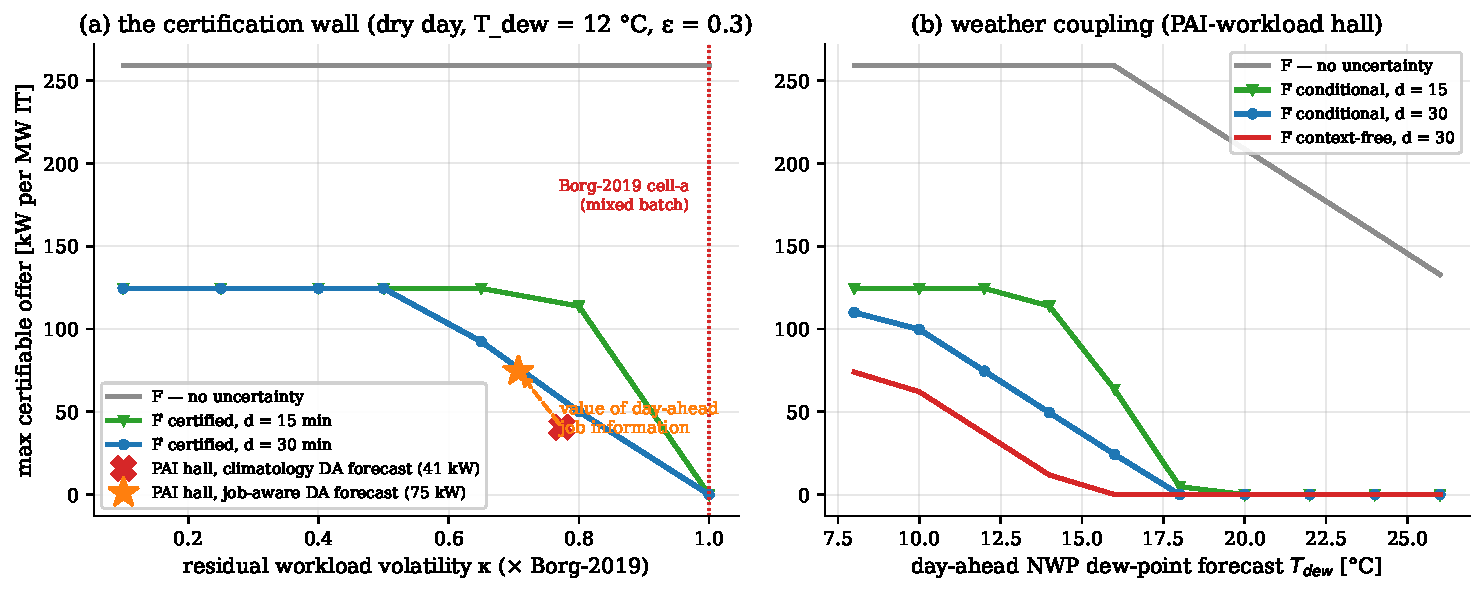
\includegraphics[width=\textwidth]{F1_context}
\caption{The certified S2 envelope on real data ($d=30$\,min, $\epsd=0.3$,
$\epss=0.05$). (a)~Certified offer vs.\ residual workload volatility
($\times$ Borg-2019 cell-a); markers: the real PAI hall under climatology
vs.\ job-aware day-ahead forecasts --- information moves the hall along the
wall (40.7 $\to$ 74.6\,kW). (b)~Weather coupling: conditional vs.\
context-free certification vs.\ the deterministic ceiling, against the real
day-ahead NWP dew-point forecast.}
\label{fig:F1}
\end{figure*}

\subsection{Ten-Week Closed-Loop Market Results}\label{sec:cs-table}
Table~\ref{tab:main} aggregates 1{,}400 controller-days per participant.
Three observations order the comparison.

\emph{(i) Safety is the product.} B2 monetizes the most capacity (\$35.1/day
per MW$_{\mathrm{IT}}$) but violates the hotspot limit on 229 of 1{,}400
day-seeds, by up to $+9.8$\,K --- on real workload weeks, an uncertified
envelope is not a flexibility product, it is deferred downtime. B4 commits
$8\times$ less capacity, monetizes \$10.6/day, and incurs \emph{zero}
violation episodes inside its certified domain; its ten beyond-domain
excursions (statistically expected: the safety set is calibrated at
$1-\epss=95\%$) stay below $1.6$\,K, where hardware frequency scaling is the
designed backstop, versus B2's $9.8$\,K. B3's sample box lands between
(47 violation day-seeds, up to $4.9$\,K), confirming that the gap is the
guarantee, not the stochastic modeling.

\emph{(ii) Value concentrates where the grid needs it.} The scarcity week
carries the economics: B4 commits 414\,kW/day and earns \$97/day per
MW$_{\mathrm{IT}}$ during Winter Storm Heather, near the price ceiling that
even the unconstrained B2 attains. Averaged across all ten weeks the certified
value is \$10.6/day ($\approx$\$3.9k/MW-yr): 2024 ERCOT capacity prices
outside scarcity hours are a few \$/MWh, so the \emph{ceiling} for any
strategy is B2's \$35. Cooling-side flexibility is a scarcity asset, and that
is the correct shape for a resource whose marginal cost is thermal-comfort
risk.

\emph{(iii) Zero capex, zero workload impact.} Scaled to a 100\,MW AI campus,
the certified product is worth $\approx$\$390k/yr using hardware the facility
already owns. The battery (B5) returns less (\$6.5/day) before its capital
cost is even counted; workload curtailment (B6) returns more (\$25.6/day) but
prices direct interference with the compute product, which the cooling-side
resource never touches. The two are complements in a portfolio; only the
cooling loop is free.

\begin{table}[!t]
\centering
\caption{Ten ERCOT 2024 weeks $\times$ 20 seeds (1{,}400 day-seeds each),
per MW$_{\mathrm{IT}}$. MV: market value vs.\ B1. Violations: hotspot
day-seeds (max excursion).}
\label{tab:main}
\begin{tabular}{lccccc}
\toprule
 & MV & Committed & Delivery & Penalty & Violations \\
 & \$/day & kW/day & ratio & \$/day & days (max K) \\
\midrule
B2 naive          & 35.1 & 388 & 0.82 & 1.49 & 229 (9.8) \\
B3 SAA            & 14.9 & 126 & 0.97 & 0.25 & 47 (4.9) \\
\textbf{B4 (ours)} & \textbf{10.6} & \textbf{54} & \textbf{0.95} &
\textbf{0.17} & \textbf{0 in-domain (1.6)} \\
B5 battery        &  6.5 & 616 & 1.00 & 0    & 0 \\
B6 curtailment    & 25.6 & 333 & 1.00 & 0    & 0 \\
\midrule
\multicolumn{6}{l}{\footnotesize B4 scarcity week: \$97.1/day at 414 kW/day
committed; delivery ratio 0.92.}\\
\bottomrule
\end{tabular}
\end{table}

\subsection{Certificate Validation}\label{sec:cs-cert}
Theorem~\ref{thm:guarantee}\todo{ref to Sec.~VI} makes two falsifiable claims,
and the held-out replay tests both at the design point $\epsd=0.3$.
\emph{Safety:} across 1{,}400 day-seeds, no violation episode starts in an
hour whose realized disturbance lies in the calibrated safety set
$\Wsafe(c)$ --- zero in-domain episodes, against the theorem's
``for all $w \in \Wsafe$'' clause. \emph{Delivery:} of 122 activated
obligations, 24 fell short (19.7\%, within the priced budget
$\epsd = 0.3$); every failure is attributable to a warm start at the envelope
boundary covered by the $e_0$-ball analysis of
Lemma~\ref{lem:e0}\todo{ref}, and \emph{none} occurred on a cold start with
in-set disturbances (0 of 22; exact 95\% Clopper--Pearson upper bound 15.4\%).
At the conservative frontier point $\epsd = 0.1$ the observed failure rate is
12.7\% against a larger disturbance set, with market value \$9.1/day ---
the $\epsd$ frontier trades certified depth against priced delivery risk, and
the settlement internalizes the trade through the $\gamma$-penalty.
Three adversarial stress days designed \emph{outside} every calibrated set
(all-hours top-decile bursts, $+3$\,K systematic dew shift, six consecutive
activations) bound the failure mode: B4's worst excursion is $2.2$\,K with
penalties of a few \$/day, versus B2's $5.1$--$6.9$\,K.

\subsection{Degradation-Cost Sensitivity}\label{sec:cs-f3}
Fig.~\ref{fig:F3} sweeps the lifetime-cost coefficient $c_{\mathrm{deg}}$
over two orders of magnitude. The certified commitment contracts smoothly
from 1{,}368 to 498\,kW on the scarcity day (value \$867 $\to$ \$445/day) and
exits the market entirely on the mild day beyond
$c_{\mathrm{deg}} \approx 20$\,\$/K$\cdot$h: a hall whose operator prices
silicon wear conservatively self-selects out of low-price hours but remains a
scarcity resource. The supply curve an aggregator would see is therefore
well-behaved --- monotone, smooth, and price-elastic at exactly the hours the
grid values least.

\begin{figure}[!t]
\centering
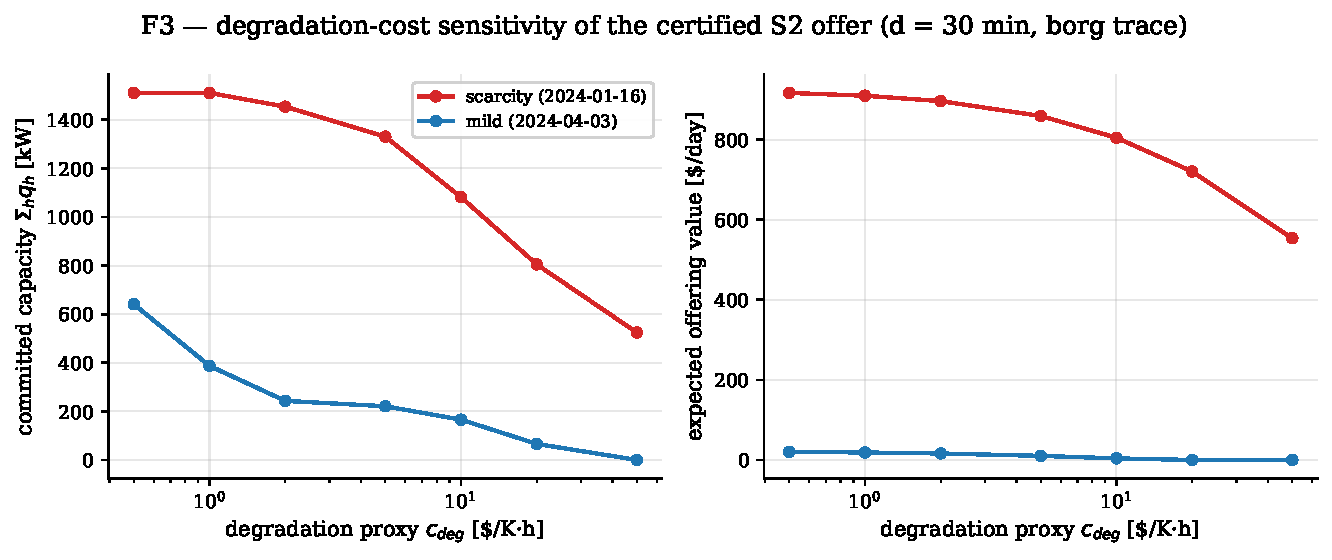
\includegraphics[width=\columnwidth]{F3_cdeg}
\caption{Degradation-cost sensitivity of the certified daily commitment
(scarcity vs.\ mild day; $d=30$\,min). Monotone contraction; the mild day
exits beyond $c_{\mathrm{deg}}\!\approx\!20$\,\$/K$\cdot$h.}
\label{fig:F3}
\end{figure}

% =====================================================================
\section{Limitations and Outlook}\label{sec:limits}
\todo{Sec.~VIII drafted last with abstract: duration parameter $d$; chiller-assist
topology assumption; metering point; DVFS backstop sentence; price-limited average
value; future: $d{=}15$ layering, affine disturbance feedback, per-context gains.}

% =====================================================================
\bibliographystyle{IEEEtran}
\begin{thebibliography}{28}
% Curated budget: <=30 (paper/REFS_VERIFIED.md is the source of truth).
% Only entries cited so far are filled; remaining slots reserved by key.

\bibitem{gheni26} \todo{Gheni et al., 2026, Applied Energy — exact bib from
REFS\_VERIFIED at compile.}

\bibitem{weng22} Q.~Weng \emph{et al.}, ``{MLaaS} in the wild: Workload
analysis and scheduling in large-scale heterogeneous {GPU} clusters,'' in
\emph{Proc. USENIX NSDI}, 2022.

\bibitem{tirmazi20} M.~Tirmazi \emph{et al.}, ``Borg: The next generation,''
in \emph{Proc. ACM EuroSys}, 2020.

% Reserved keys (Secs. I-VI): takci25, colangelo25, acun26, oh25, zhang25,
% ravi26, chen23, fanzhao26, ghatikar12, fu20, wierman14, vrettos16tse,
% vrettos16tps, gorecki17, zhao15dne, doe-envelopes, hao15, junker18,
% warrington13, baselinegaming, lei18, norris25, sb6, googledr, e2ecdro
\end{thebibliography}

\end{document}
